%\subsection{Det Abstrakte syntakstræ}
%\begin{frame}
%  \frametitle{Det Abstrakte syntakstræ}

%  \begin{figure}
%    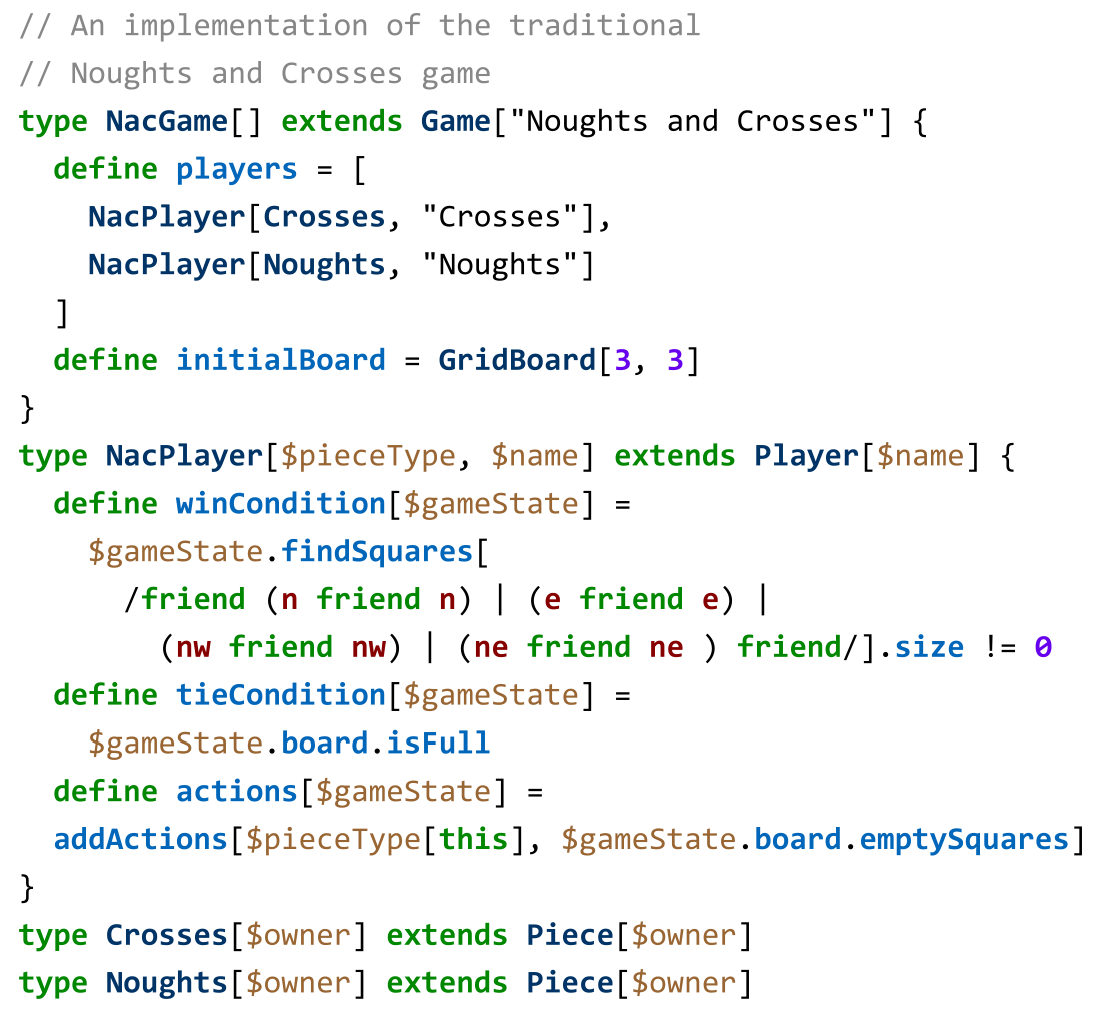
\includegraphics[width=0.6\linewidth]{billeder/krydsogbolle}
%  \end{figure}
%\end{frame}

\begin{frame}
  \frametitle{Det Abstrakte syntakstræ}
 
  \input{billeder/tikz/typedef}



  
\begin{figure}[ht]
  \begin{center}\scalebox{0.7}{
\begin{tikzpicture}[level/.style={sibling distance=30mm/#1}]
\node [square] {Element}
  child {node [square, xshift=-1cm] {Call sequence}}
  child {node [square, xshift=-0.3cm] {Member access}}
  child {node [square,xshift=0.3cm] (b) {Member access} edge from parent[dashed]}
  child {node [square,xshift=1cm] (c) {Member access} edge from parent[dashed]};
  
\path (b)--(c) node [midway] {$\cdots$};
\end{tikzpicture}}
\end{center}
\end{figure}

  \begin{figure}[ht]
\begin{center}
\begin{tikzpicture}[level/.style={sibling distance=30mm/#1}]
\node [square] {Constant definition}
  child {node [square,xshift=0.7cm] {Constant}}
  child {node [square] {Variable list} edge from parent [dashed]}
  child {node [square,xshift=-0.7cm] {\textit{Expression}}};
\end{tikzpicture}
\end{center}
\capt{The abstract syntax tree for the constant definition node.}
\label{ast:constdef}
\end{figure}

\end{frame}

\begin{frame}
  \frametitle{Det Abstrakte syntakstræ}

  \begin{itemize}
    \item Vokser meget hurtigt
    \item Komprimere træet så godt som muligt
      \begin{itemize}
        \item Fjerne unødvendige knuder
        \item Gør det videre arbejde med træet nemmere
      \end{itemize}
  \end{itemize}
\end{frame}

